\documentclass{article}
\usepackage{times}
\usepackage{subfigure}
\usepackage{algorithm}
\usepackage{algorithmic}
\usepackage{multirow}
\usepackage{hhline}
\newcommand{\theHalgorithm}{\arabic{algorithm}}
\usepackage{icml2015} 
\RequirePackage[OT1]{fontenc}
\RequirePackage{amsthm,amsmath,amssymb}
\usepackage{ifpdf}
\usepackage{graphicx}
\usepackage{epsf}
\usepackage{natbib}
\RequirePackage{hyperref}
\usepackage[small,compact]{titlesec}
\allowdisplaybreaks[4]
\usepackage{setspace}
%\setlength{\textwidth}{6in} 
 \setlength{\textwidth}{27pc}
 \usepackage[margin=1in]{geometry}
% \setlength{\textheight}{8.5in}
% \setlength{\topmargin}{-.5in}
% \setlength{\oddsidemargin}{.25in}
%\doublespacing 

\numberwithin{equation}{section}
\theoremstyle{plain}
%% Need to site http://julia-e-vogt.com/Publications_files/DAGM2010.pdf
%% http://arxiv.org/ftp/arxiv/papers/1206/1206.4632.pdf
%% Include reference to OSCAR and this
% http://www.icml-2011.org/papers/9_icmlpaper.pdf
% http://arxiv.org/ftp/arxiv/papers/1206/1206.4601.pdf

\newtheorem{thm}{Theorem}[section]
\newtheorem{prop}{Proposition}[section]
\newtheorem{defn}{Definition}[section]
\newtheorem{lem}{Lemma}[section]
\newtheorem{corr}{Corollary}[section]
\newtheorem{claim}{Claim}[section]
\newtheorem{rem}{Remark}[section]

\newcommand{\bs}{\boldsymbol}
\newcommand{\OLS}{\mbox{OLS}}

%\title{The Sparse Spatial Group LASSO}
\icmltitlerunning{The Sparse Spatial Group LASSO}

\begin{document}

\twocolumn[
\icmltitle{The Sparse Spatial Group LASSO}
\icmlauthor{Daniel V Samarov}{daniel.samarov@nist.gov}
\icmladdress{
Statistical Engineering Division,
National Institute of Standards and Technology,
Gaithersburg, MD 20899
}
\icmlkeywords{LASSO, group sparsity, multivariate statistics, spatial
statistics}

\vskip 0.3in
] 
% \author{ 
% Daniel V. Samarov \footnote{Daniel V. Samarov
% is a Mathematical Statistician, Statistical Engineering Division, Information
% Technology Laboratory, National Institute of Standards and Technology (NIST),
% Gaithersburg, MD 20899, (Email:
% daniel.samarov@nist.gov).
%   }}



\begin{abstract}

In many applications the grouping of covariates naturally arises as does
sparsity at both the group and within group levels. To address this approaches
using $l_2$ and $l_1$ penalties have been developed. While these methods address
the sparsity component of the problem when there is a
sense of spatial (or neighborhood) coherence between coefficients it is
desirable to effectively leverage this information to improve our estimates. In
this work we propose a novel model which incorporates both group and
elementwise sparsity along with spatial information in the form of a graph
Laplacian based penalty to help improve the model estimation process. We show
the strong performance of this model on both simulated and real data.

\end{abstract}

\section{Introduction}
\label{SEC:INTRO}

% In many regression applications parameter estimation can be greatly improved
% through the inclusion of spatial/neighborhood information.
In regression applications the process of identifying variables most predictive
of the outcome is critical for avoiding issues involving over-fitting,
helping to improve prediction on new data and assisting in overall model
interpretability.
When the number variables is large this problem becomes particularly
challenging. 
To help address these multiple challenges $l_1$-norm based penalized regression
models, such as the LASSO (\cite{tibs96lasso}) have become
increasingly popular.
% To assist in the process of identifying the subset of
% variables most predictive of outcome $l_1$-norm based penalized regression
% models, such as the well known LASSO (\cite{tibs96lasso}) have become
% increasingly popular.
%  To
% address this the well known LASSO,
% \cite{tibs96lasso} introduces an $l_1$-norm penalty on the coefficients vector
% $\bs\beta$. 
Letting $\mathbf{X} \in \mathbb{R}^{n \times p}$ be the data
matrix, and $\bs\beta \in \mathbb{R}^p$ and $\mathbf{y} \in \mathbb{R}^n$ the
vectors of coefficients and responses, respectively the LASSO minimizes
\begin{align}
\label{EQ:LASSO}
\mathcal{L}(\mathbf{y}, \mathbf{X}, \bs\beta, \gamma) = \frac{1}{2}||\mathbf{y}
- \mathbf{X}\bs\beta||_2^2 + \gamma ||\bs\beta||_1,
\end{align}
\noindent with respect to $\bs\beta$. Here $||\mathbf{u}||_q = (\sum_{j=1}^p
u_j^{q})^{1/q}$, $q > 0$ denotes the $q$-norm and $\gamma \geq 0$ is a regularization
parameter.
For sufficiently large values of $\gamma$,
(\ref{EQ:LASSO}) will yield solutions with some/many zero entries in $\bs\beta$,
effectively removing these variables from the model. 

Taking this a step further to the multivariate regression setting, suppose that
we have multiple outcomes $\mathbf{y}^{(k)} \in \mathbb{R}^{n_k}$, $k = 1,
\ldots, K$ with corresponding data matrices and coefficient vectors,
$\mathbf{X}^{(k)} \in \mathbb{R}^{n_k \times p}$ and $\bs\beta^{(k)} \in
\mathbb{R}^p$. Letting $\mathcal{L}_k = \mathcal{L}(\mathbf{y}^{(k)},
\mathbf{X}^{(k)}, \bs\beta^{(k)}, \gamma_k)$ a direct extension of
(\ref{EQ:LASSO}) leads to
\begin{align}
\label{EQ:MLASSO}
\sum_{k=1}^K \mathcal{L}_k
\end{align}
\noindent amounting to fitting $K$ separate LASSO models. 

However, in many instances it is of interest to understand the relevance of the
$j^{th}$ variable {\it across} all $K$ responses. Specifically, letting
$\bs\beta_j = (\beta^{(1)}_j, \ldots, \beta^{(K)}_j)$, be the coefficient
estimates across outcomes for the $j^{th}$ variable, we want to determine
whether $\bs\beta_j = \mathbf{0}$ or $\bs\beta_j \neq \mathbf{0}$, where
$\mathbf{0}$ is a $p$-vector of 0's. 


An example of where this type of behavior is of interest is in dictionary
learning type applications, such as abundance estimation in hyperspectral image
(HSI) analysis.
% (additional discussion in Section \ref{SEC:RES}).
% In HSI, specialized cameras and microscopes collect series of images at
% specific wavelengths (densely sampled) over a range of interest along the
% electromagnetic spectrum (ES). The resulting set of images are then
% ``stacked'' together (in order of wavelength) to form a three-dimensional HSI
% data cube.
% Because many objects, from the molecular level up, exhibit unique spectral
% signatures (referred to as endmembers), HSI can be used to identify various
% targets of interest in an image based on their spatial and spectral
% distributions.
% However, due to limitations in camera resolution, scattering artifacts and
% other factors related to the physical/chemical composition of the object(s)
% being imaged each pixel in a HSI is frequently composed of not just one, but
% several endmembers.
In HSI we have $n$, $M \times N$ images stacked one after another (forming a so
called ``hyperspectral data cube''), where each image represents the
reflectance/absorbance measurements at a given wavelength (ordered from smallest
to largest) along the electromagnetic spectrum (ES). With a total of $K = M
\times N$ pixels (i.e. outcomes) the spectral signature/response at pixel $k$ is
denoted by $\mathbf{y}^{(k)} \in \mathbb{R}^n$, here $n$ denotes the number of
wavelengths measured along ES with each element corresponding to a reflectance
or absorbance intensity measurement.

How HSI ties into regression type frameworks is that each spectral response is
assumed to be composed of $p$ ``pure'' spectral signatures (also called
``endmembers'') so that $\mathbf{y}^{(k)} = \sum_{j=1}^p \mathbf{X}
\bs\beta^{(k)} + \bs\epsilon^{(k)} \in \mathbb{R}^n$, $k = 1,\ldots,K$. Here
$\mathbf{X} \in \mathbb{R}^{n \times p}$ is a matrix whose columns contain these
endmembers, $\bs\beta^{(k)} = (\beta_1^{(k)}, \ldots, \beta_p^{(k)})$,
$\beta_j^{(k)} \geq 0$ is the coefficient vector of associated ``abundances'' of
each of those endmembers at location corresponding to pixel $k$ and
$\bs\epsilon^{(k)} = (\epsilon_1^{(k)}, \ldots, \epsilon_p^{(k)})$ is i.i.d
noise.
This is referred to as the linear mixing model, for additional details see
\cite{dias2011}, \cite{clarke2011}, \cite{clarke2012}, \cite{samarov2012boe}.
 

Since not every pixel will contain every endmember the LASSO is a natural fit.
Furthermore, in many instances ``overcomplete'' dictionaries of endmembers are
used, with some or many not present in the image at all. As such methods that
can simultaneously determine the presence of endmembers within a pixel, as well
as {\it across} pixels are needed. Note that in HSI the matrix of endmembers,
$\mathbf{X}$ is taken to be the same across pixels.


To capture this ``structured'' sparsity \cite{yuan06} developed the group LASSO
(GL). The GL places an $l_2$-norm penalty on the coefficient vector
$\bs\beta_j$, so that the loss function becomes
\begin{align}
\label{EQ:GLASSO}
\sum_{k=1}^K
\left[ 
\frac{1}{2}||\mathbf{y}^{(k)} - \mathbf{X}^{(k)}\bs\beta||_2^2
\right]
+
\sum_{j=1}^p\mathcal{P}_2^{j}(\lambda).
\end{align}
\noindent where $\mathcal{P}_2^{j}(\lambda) = \lambda
||\bs\beta_j||_2$. The introduction of $||\bs\beta_j||_2$ has the effect of
shrinking the {\it entire} coefficient vector to 0 for sufficiently large
values of the regularization parameter $\lambda$. 

While not implemented in the examples presented in this paper, it is worth
noting that the sum in (\ref{EQ:GLASSO}) for the group penalty term can also be
a sum over a more general grouping index, i.e. rather having $j \in \{1, \ldots,
p \}$, have $j \in \{\mathcal{G}_1, \ldots, \mathcal{G}_{n_g} \}$, where
$\mathcal{G}_j$ denotes a collection of indices associated with our
$\beta_j^{(k)}$'s. Furthermore, overlaps in the $\mathcal{G}_j$'s is allowed,
though some certain adjustments need to be made, see \cite{jacob2009} for
discussion.
 
An interesting property is that
for {\it all} $l_q$-norms, $q > 1$ the same type of group sparse behavior as
in (\ref{EQ:GLASSO}) is achieved (see \cite{vogt2012}).
In the case where $\bs\beta_j \neq 0$ for $q \approx 2$ the behavior of the coefficient
estimates resembles that of ridge regression, \cite{hastie2009},
\cite{simon2013}. On the opposite extreme, as $q \rightarrow \infty$
coefficient estimates tend to collapse to the same value, 
referred to as the ``tight-coupling'' effect by \cite{vogt2012}.

The benefit of the $l_2$-norm over the $l_{\infty}$-norm is that there tends to
be less shrinkage, and as a result less bias in the coefficient estimates from
the introduction of the penalty term.
However, when there are noisy and/or outlying observations $\mathbf{y}^{(k)}$,
the $l_{\infty}$-norm tends to be less impacted as far as identifying the ``true''
underlying subset of sparse coefficient vectors (see \cite{sgen2014} for
discussion and examples).

One potential shortcoming of the GL model is that while it allows us to identify
group-wise sparse structure in our coefficients we sacrifice the ability to
produce element-wise sparsity, i.e.
if $\bs\beta_j \neq 0$, then $\beta_j^{(k)} \neq 0$, $\forall k \in
\{1,\ldots,K\}$. To address this \cite{simon2013} introduced the sparse GL (SGL)
model defined as,
\begin{align}
\label{EQ:SGL}
\sum_{k=1}^K \mathcal{L}_k
+ 
\sum_{j=1}^p\mathcal{P}_2^{j}(\lambda).
\end{align}
\noindent i.e. the combination
of the standard LASSO with the
$l_2$-norm group penalty. Similar work has been done looking at the combination
of $l_{\infty}$ and $l_1$ penalties, \cite{sgen2014}.
% The SGL model provides an additional level of flexibility allowing for various
% forms of sparsity to be effectively captured.
% The methods we have described to this point allow us to model various types of
% sparsity, however, in many applications we also have spatial (or neighborhood)
% information available to us.
As will be discussed in Section \ref{SEC:RES} for HSI analysis both forms of
sparsity (group and element-wise) are important in order to reliably identify
the dictionary elements present in an image and, for those that are, their
quantity (or ``abundance'') at each pixel.

In addition to the wide range of complex, sparse coefficient structures the SGL
model allows us to capture, there are also many applications where neighborhood
information is available or can otherwise be derived.
% While the SGL model allows us capture a wide range of complex sparse
% structures in our coefficient estimates, in practice there are also many
% applications where we also have ``neighborhood'' information available to us.
For example, in HSI applications neighborhoods are typically described as
spatially proximal pixels. In principle those pixels near one another should
have similar abundance estimates. By effectively leveraging this information we
can help improve the accuracy of our estimates and their robustness to noise. In
what follows we introduce a novel model called the sparse spatial group LASSO
(SSGL) that combines both element and group-wise sparsity with a spatial
constraint encouraging points ``near'' one another to have similar coefficient
estimates.

In Section \ref{SEC:BACK} we begin by providing background on the conditions for
group sparsity and the spatial LASSO (SPLASSO), \cite{samarov2014splasso}, in
Section \ref{SEC:SSGL} we introduce the SSGL model, in Section \ref{SEC:SOL} we
provide a coordinate descent based approach for solving the SSGL and finally in
Section \ref{SEC:RES} we provide results on both simulated and real world HSI
examples.

\section{Background}
\label{SEC:BACK}


\subsection{Group Sparsity Conditions}
\label{SEC:GSC}

We begin by describing the standard GL model to provide some intuition and
background on group sparsity. Coming back to the optimization problems for the
GL shown in (\ref{EQ:GLASSO}) we note that the objective function is
convex and as such the optimal solution can be characterized by its
subgradient equations (as the $l_2$ norm is 
non-differentiable at 0). For 
a given $j$ (fixing remaining $l \neq j$) we have
\begin{align}
\label{EQ:SUBG0}
(\mathbf{y}^{(k)} - \sum_{l=1}^p \mathbf{x}^{(k)}_l\beta_l^{(k)})^T
\mathbf{x}^{(k)}_j = \lambda \eta_k, k = 1,\ldots,K.
\end{align}
\noindent where $\mathbf{x}_l^{(k)}$ denotes the $l^{th}$ column of
$\mathbf{X}^{(k)}$ and $\bs\eta = (\eta_1, \ldots, \eta_K)$ denotes the
subgradient of $||\hat{\bs\beta}_j||_2$. 
For the $l_2$-norm
\begin{align}
\label{EQ:L2_DIFFL}
\bs\eta = 
\left\{
\begin{array}{cc}
\frac{\hat{\bs\beta}_j}{||\hat{\bs\beta_j}||_2} & \mbox{if } \hat{\bs\beta}_j
\neq
\mathbf{0}
\\
\{\bs\eta: ||\bs\eta||_2 \leq 1 \} & \mbox{if } \hat{\bs\beta}_j =
\mathbf{0}.
\end{array}
\right.
\end{align}
Taking a closer look, let $\mathbf{r}_j^{(k)} = \mathbf{y}^{(k)} - \sum_{l
\neq j} \mathbf{x}^{(k)}_l \hat{\beta}_l^{(k)}$ denote the partial residual
vector, the
subgradient equations are satisfied when
\begin{align}
\label{EQ:GTH_L2}
\sqrt{\sum_{k=1}^K (\mathbf{x}^{(k)T}_j \mathbf{r}_j^{(k)})^2} \leq \lambda,
\end{align}
\noindent see \cite{simon2013} and \cite{friedman2010note}
for details on these derivations.

When  
$\hat{\bs\beta}_j \neq \mathbf{0}$ holding the remaining $\bs\beta_l$, $l \neq
j$ coefficient vectors fixed,
let $\alpha_j^{(k)} = \mathbf{x}^{(k)T}_j \mathbf{r}_j^{(k)}$, $d^{(k)}_{ij} =
\mathbf{x}_i^{(k)T} \mathbf{x}^{(k)}_j$ . 
It
can be shown that for a particular $j$ and $k$ the
solution to the GL model is
\begin{align}
\label{EQ:B_GL}
\hat{\beta}_j^{(k)}(GL) = \frac{\alpha_j^{(k)}}{d^{(k)}_{jj} +
\lambda/||\hat{\bs\beta}_j||_2} 
% \cdot \mathbf{1}_{\{ ||\bs\alpha_j||_2 \geq \lambda \}}
\end{align}
\noindent where $\bs\alpha_j = \{\alpha_j^{(k)}\}_{k=1}^K$. From
(\ref{EQ:B_GL}) we can see blockwise-coordinate descent (BCD),
\cite{nonlin1999}, \cite{tseng2001} as
a natural approach to minimizing the loss functions. 

Next, consider the extention of the GL to the SGL model proposed by
\cite{simon2013}. Letting
$S(u, v) = \mbox{sign}(u)(|u| - v)_+$ denote the
soft thresholding operator, where $(u)_+ = \max\{0, u\}$ 
(\ref{EQ:GTH_L2}) is modified to be
\begin{align}
\label{EQ:SGTH_L2}
\sqrt{\sum_{k = 1}^K S(\alpha_j^{(k)}, \gamma_k)^2} \leq \lambda
\end{align}
\noindent and (\ref{EQ:B_GL}) becomes
\begin{align}
\label{EQ:B_SGL}
\hat{\beta}_j^{(k)}(SGL) = \frac{S(\alpha_j^{(k)}, \gamma_k)}{d^{(k)}_{jj} +
\lambda/||\hat{\bs\beta}_j||_2}.
%\cdot \mathbf{1}_{\{ ||\bs\alpha_j||_2 \geq \lambda \}}
\end{align}
\noindent As can be seen the primary difference between the GL and SGL models is
that for the case where $\hat{\bs\beta}_j \neq 0$ we now have element-wise sparsity. 

With a general understanding of how the $l_2$-norm penalty works we now provide
an overview of the SPLASSO.

\subsection{Spatial LASSO}
\label{SEC:SPLASSO}

While the GL and SGL models allow us to capture group sparse structure in our
coefficient estimates there are many applications where leveraging spatial
information is also of value. The SPLASSO model does this
via a graph Laplacian based penalty of the form
\begin{align}
\label{EQ:SPPEN}
\mathcal{P}_s^{k}(\rho) = \frac{\rho}{2}\sum_{l \in
N(\mathbf{y}^{(k)})} ||\bs\beta^{(k)} - \bs\beta^{(l)}||_2^2 w_{kl}.
\end{align}
\noindent Here $N(\mathbf{y}^{(k)})$ denotes the set of
neighboring points about $\mathbf{y}^{(k)}$ and $w_{kl}$ is the weight
controlling the degree to which $\hat{\bs\beta}^{(k)}$ is ``encouraged'' to be
similar to $\bs\beta^{(l)}$. 
In image analysis applications, such as HSI $N(\cdot)$ is frequently
taken to be the $k$-neighborhood about the $(i,j)^{th}$ pixel, e.g. for $k = 1$
we would have $\{ (i-1,j-1), (i-1,j), (i-1,j+1), (i,j-1), (i,j+1), (i+1,j-1), (i+1,j),
(i+1,j+1)\}$ as the set of neighbors. 


The inclusion of (\ref{EQ:SPPEN}) into our model has the effect of introducing a
spatial smoothness to the coefficients. This allows our estimates to be
more robust to various sources of noise as these will tend to be smoothed out.
Of course, as with any type of smoothing, care needs to be taken to avoid
removing features actually present or adding those that are not. As such the
choice of the weights $w_{kl}$ is extremely important. 

For example, in the
context of HSI a similarity metric commonly used is the cosine of the angle
between spectra, $\cos(\theta_{kl}) = \mathbf{y}^{(k)T} \mathbf{y}^{(l)} /
(||\mathbf{y}^{(k)}||_2 ||\mathbf{y}^{(l)}||_2)$ with some cutoff so that
$w_{kl} = 0$ for $\cos(\theta_{kl}) < \tau$, $\tau \in (0, 1)$. This metric can
then be used as our spatial weight function, i.e. $w_{kl} = \cos(\theta_{kl}) \cdot
1_{\{ \cos(\theta_{kl}) \geq \tau \}}$, where $1_{\{ \cdot \}}$ is the
indicator function.
As there is considerable information about the composition of the various
elements in a given pixel based on the spectral response this weight function
tends to perform well in most circumstances. 


Putting together (\ref{EQ:SPPEN}) and (\ref{EQ:MLASSO}) the SPLASSO loss
function is expressed as
\begin{align}
\label{EQ:SPLASSO}
\sum_{k=1}^K \mathcal{L}_k
+ \mathcal{P}_s^{k}(\rho).
\end{align}
\noindent Two approaches to solving (\ref{EQ:SPLASSO}) are
least angle regression (LARS) and 
BCD, \cite{lars2004} , \cite{samarov2014splasso}. We
focus on the latter as it provides insight into how the SPLASSO works
and fits in with the proposed solution to the SSGL model described in Section
\ref{SEC:SSGL}. 

Letting $b_j^{(k)} = \alpha_j^{(k)} + \rho \sum_{l \in N(\mathbf{y}^{(k)})}
\beta_j^{(l)}w_{kl}$ our BCD update is
\begin{align*}
\beta_j^{(k)} = 
\frac{S(b_j^{(k)}, \gamma_k)}{d^{(k)}_{jj} + \rho \sum_{l \in
N(\mathbf{y}^{(k)})} w_{kl}}.
\end{align*}
\noindent This is essentially a weighted average between the least squares
estimate, $\alpha_j^{(k)}$ and its neighbors controlled by the regularization
parameter $\rho$. 

% As part of future work we plan to also look into the use of ``Total Variation''
% type penalties, i.e. $||\bs\beta^{(k)} - \bs\beta^{(l)}||_1$. These have been
% shown to be quite effective in a number of applications (\cite{tibs2005},
% \cite{io2012}) and tend to oversmooth less than the $l_2$ type penalty used
% here.

\section{The Sparse Spatial Group LASSO}
\label{SEC:SSGL}

Using the results from Sections \ref{SEC:GSC} and \ref{SEC:SPLASSO} the SSGL
model can be expressed as
\begin{align}
\label{EQ:SSGL}
\sum_{k=1}^K \left[ \mathcal{L}_k
+ \mathcal{P}_s^{k}(\rho) \right] + \sum_{j=1}^p\mathcal{P}_2^{j}(\lambda).
\end{align}
\noindent This combines the GL and SPLASSO models, allowing us to leverage
spatial information as well as group and element-wise sparsity.  For a given
$j$, fixing the remaining $l \neq j$, the subgradient equations for
(\ref{EQ:SSGL}) can be expressed as
\begin{align}
\label{EQ:SUBG1}
% (\mathbf{y}^{(k)} & - \sum_{l=1}^p \mathbf{x}^{(k)}_l\beta_l^{(k)})^T
% \mathbf{x}^{(k)}_j = 
% \lambda \eta_k + \gamma \nu_j^{(k)} \nonumber \\
% & + \rho \sum_{l \in N(\mathbf{y}^{(k)})}
% \left( 
% \beta_j^{(l)} -
% \beta_j^{(k)}
% \right) w_{kl}.
b_j^{(k)} & - c_j^{(k)} \beta_j^{(k)}
% (\mathbf{y}^{(k)} & - \sum_{l=1}^p \mathbf{x}^{(k)}_l\beta_l^{(k)})^T
% \mathbf{x}^{(k)}_j
 = 
\lambda \eta_k + \gamma_k \nu_j^{(k)} 
% & + \rho \sum_{l \in N(\mathbf{y}^{(k)})}
% \left(
% \beta_j^{(k)} - \beta_j^{(l)}
% \right) 
% w_{kl}.
\end{align}
\noindent where 
\begin{align}
\label{EQ:SPDEN}
c_j^{(k)} = d_{jj}^{(k)} + \rho \sum_{l \in
N(\mathbf{y}^{(k)})} w_{kl}. 
\end{align}
\noindent Here $\nu_j^{(k)}$ is the subderivative of
$|\hat{\beta}_j^{(k)}|$ and takes values
\begin{align}
\label{EQ:SG_L1}
\nu_j^{(k)} =
\left\{
\begin{array}{cc}
\mbox{sign}(\hat{\beta}_j^{(k)}) & \mbox{if } \hat{\beta}_j^{(k)} \neq 0 \\
\in \{\nu_j^{(k)}: |\nu_j^{(k)}| \leq 1 \} & \mbox{if } \hat{\beta}_j^{(k)} =
0,
\end{array}
\right.
\end{align}
\noindent and $\nu_k$ is the same as in (\ref{EQ:L2_DIFFL}). 

To gain insight into the behavior of our model and derive the quantities that
will be needed to solve (\ref{EQ:SSGL}) we consider the cases where
$\bs\beta_j = \mathbf{0}$ or $\bs\beta_j \neq \mathbf{0}$ and $\beta_j^{(k)} =
0$ for some $k$ or $\beta_j^{(k)} \neq 0$.
Starting with $\bs\beta_j = \mathbf{0}$ and following the discussion of
\cite{friedman2010note} we have that the system of equations
\begin{align}
\label{EQ:ZERO}
b_j^{(k)} 
 = 
\lambda \eta_k + \gamma_k \nu_j^{(k)},
\end{align}
\noindent must 
satisfy $\nu_j^{(k)} \in [-1, 1]$ and $||\bs\eta||_2 \leq
1$, where $\bs\eta = (\eta_1, \ldots, \eta_K)$. This can be shown by minimizing 
\begin{align}
\label{EQ:ZERO_MIN}
\frac{1}{\lambda^2} \sum_{k = 1}^K (b_j^{k} - \gamma_k
\eta_j^{(k)})^2 = \sum_{k = 1}^K \eta_k^2,
\end{align}
\noindent with respect to $\eta_j^{(k)}$, $k = 1,\ldots,K$. Straightforward
calculations give us that (\ref{EQ:ZERO_MIN}) is solved by
\begin{align}
\label{EQ:ZERO_ETA}
\nu_j^{(k)} =
\left\{
\begin{array}{ll}
\frac{b_j^{(k)}}{\gamma_k} & \mbox{if } |b_j^{(k)}/\gamma_k| \leq 1, \\
\mbox{sign}\left(\frac{b_j^{(k)}}{\gamma_k}\right) & \mbox{if }
|b_j^{(k)}/\gamma_k| > 1,
\end{array}
\right.
\end{align}
\noindent which clearly satisfies the condition $\eta_j^{(k)} \in [-1, 1]$ and
$||\bs\eta||_2 \leq 1$ follows directly from (\ref{EQ:L2_DIFFL}). Re-arranging
terms in (\ref{EQ:ZERO_MIN}) and combining with (\ref{EQ:ZERO_ETA}) shows us
that $\bs\beta_j = \mathbf{0}$ when $\sqrt{\sum_{k = 1}^K S(b_j^{(k)},
\gamma_k})^2 \leq \lambda$.

On the other hand when $\bs\beta_j \neq \mathbf{0}$ we have
\begin{align}
\label{EQ:NZERO}
b_j^{(k)} - c_j^{(k)} \beta_j^{(k)}
 = 
\lambda \frac{\beta_j^{(k)}}{||\bs\beta_j||_2} + \gamma_k \nu_j^{(k)}.
\end{align}
\noindent When $\beta_j^{(k)} = 0$ the subgradient conditions are satisfied
when 
$|b_j^{(k)}| \leq \gamma.$
On the other hand when $\beta_j^{(k)} \neq 0$ then
\begin{align*}
\beta_j^{(k)} =
\frac{S(b_j^{(k)}, \gamma_k)}{c_j^{(k)} + \lambda/||\bs\beta_j||_2}.
\end{align*} 
\noindent Similar to the GL and SGL models the SSGL has ridge
regression like behavior in its non-zero coefficient estimates. However,
particular care needs to be taken as our parameters are being shrunk
by both the group sparse parameter, $\lambda$ and the spatial parameter
$\rho$. As such it is often desirable to let $\lambda$ vary with $j \in
\{1,\ldots,p\}$, i.e. take $\lambda_j = \omega_j \lambda$ where $\omega_j =
||\bs\beta_j(OLS)||_2^{-1}$ or $||\bs\beta_j(LASSO)||_2^{-1}$,
corresponding to the ordinary least squares and standard LASSO solutions
respectively, are reasonable choices (though others may be more appropriate for
a particular problem).
The idea is that if there are many small/zero coefficients for a given
$\beta_j$ then $\omega_j$ will larger, and smaller if there are many
non-zero/larger coefficients.

\subsection{Orthonormality}
Some additional insight into the behavior of the SSGL model can be made by
considering the special case of orthonormality in our design matrices, i.e.
$\mathbf{X}^{(k)T} \mathbf{X}^{(k)} = \mathbf{I}_p$, where $\mathbf{I}_p$
denotes the $p \times p$ identity matrix. Furthermore, for illustrative purposes
let us assume that $\sum_{l \in N(\mathbf{y}^{(k)})} w_{kl} = 1$ and define
$\beta_j^{(k)}(OLS) = \mathbf{x}_j^{(k)T} \mathbf{y}^{(k)}$ and 
\begin{align}
\label{EQ:PSI}
\psi_j^{(k)} =
\sum_{l \in N(\mathbf{y}^{(k)})} \beta_j^{(l)}w_{kl} 
\end{align}
\noindent the subgradient equations
in (\ref{EQ:SUBG1}) are expressed as
\begin{align}
\label{EQ:ORTH1}
\beta_j^{(k)}(OLS) - (1 + \rho) \beta_j^{(k)} + \rho \psi_j^{(k)} = \lambda
\eta_k + \gamma_k \nu_j^{(k)}.
\end{align}
% \begin{align} \label{EQ:SSGL} \min_{\bs\beta_1,\ldots,\bs\beta_p} &
% \frac{1}{2}\sum_{k=1}^K \left(||\mathbf{y}^{(k)} -
% \mathbf{X}^{(k)}\bs\beta^{(k)}||_2^2 + \right. \nonumber \\
% & \left. \frac{\rho}{2}\sum_{l \in N(\mathbf{y}_{k})} ||\bs\beta^{(k)} -
% \bs\beta^{(l)}||_2^2 w_{kl} \right) + \lambda \sum_{j = 1}^p ||\bs\beta_j||_2
% + \gamma \sum_{j = 1}^p ||\bs\beta_j||_1, \end{align}
\noindent Dividing both sides by $1 + \rho$, define $\rho^{\ast} = 1/(1
+ \rho)$, $\lambda^{\ast} = \rho^{\ast} \lambda$ and $\gamma_k^{\ast} =
\rho^{\ast} \gamma_k$. Letting $\tilde{b}_j^{(k)} = \rho^{\ast}
\beta_j^{(k)}(OLS) + (1 - \rho^{\ast}) \psi_j^{(k)}$ (\ref{EQ:ORTH1}) can be
re-expressed as
\begin{align*}
\tilde{b}_j^{(k)} - \beta_j^{(k)} = \lambda^{\ast} \eta_k + \gamma_k^{\ast}
\nu_j^{(k)}.
\end{align*}
\noindent Following similar calculations as above and re-arranging terms we
then have
\begin{align}
\label{EQ:ORTH_SOL}
\hat{\bs\beta}_j = \frac{S(\tilde{\mathbf{b}}_j, \bs\gamma^{\ast})}{1 +
\lambda^{\ast}/||\bs\beta_j||_2}(||S(\tilde{\mathbf{b}}_j,
\bs\gamma_k^{\ast})||_2 - \lambda^{\ast})_+,
\end{align}
\noindent where $\tilde{\mathbf{b}}_j = (\tilde{b}_j^{(1)}, \ldots,
\tilde{b}_j^{(K)})$, $\bs\gamma^{\ast} = (\gamma_1^{\ast}, \ldots,
\gamma_K^{\ast})$ and $S(\tilde{\mathbf{b}}_j, \bs\gamma^{\ast}) =
(S(\tilde{b}_j^{(1)}, \gamma_1^{\ast}), \ldots, S(\tilde{b}_j^{(K)},
\gamma_K^{\ast}))$. 

With this representation we can see that (\ref{EQ:ORTH_SOL}) has the same form
as the GL and SGL models except that now our solution for $\beta_j^{(k)} \neq 0$
is a weighted average (by $\rho^{\ast} \in [0, 1]$) of the OLS estimate and it's
weighted neighbors. We can also see that the choice of $\rho$ has potentially
significant impact on both group and element-wise sparsity. Specifically, as
$\rho$ increases the level sparsity decreases without increasing $\lambda$ and
$\gamma_k$. However, as stated earlier, care needs to be taken here as
increasing the values of these parameters will compound the bias in our
coefficient estimates. In section \ref{SEC:SOL} we provide guidance on how
to select $\lambda$, $\gamma_k$ and $\rho$.

%\subsection{Other loss functions}

\section{Solving the SSGL}
\label{SEC:SOL}

Similar to the approaches in \cite{Liu2009}, \cite{fried007pco},
\cite{friedman2010note}, \cite{samarov2014splasso} and \cite{sgen2014} 
here we use a BCD based method to solve the SSGL.
Given regularization parameters $\lambda$, $\gamma_k$, $k = 1,\ldots,K$ and
$\rho$ the BCD algorithm for the SSGL problem in
(\ref{EQ:SSGL}) is given in Figure \ref{ALG:BCD}. Here each
$\hat{\bs\beta}_j$ is a block, and the algorithm consists of simultaneously
updating the coefficients within a block while holding all others fixed, then
cycling to the next block and continuing this process until convergence.
Taking the current estimates to be $\hat{\bs\beta}_l, l = 1,\ldots,p$,
$\hat{\bs\beta}_j$ is updated by computing $\alpha^{(k)}_j = \mathbf{y}^{(k)T}
\mathbf{x}_j^{(k)} - \sum_{l \neq j} \hat{\beta}_l^{(k)} d^{(k)}_{lj}$,
$\psi_j^{(k)}$ as in (\ref{EQ:PSI}) and $b_j^{(k)} = \alpha_j^{(k)} + \rho
\psi_j^{(k)}$ where we can pre-compute the quantities $h_j^{(k)} =
\mathbf{y}^{(k)T} \mathbf{x}^{(k)}_j$ and $d^{(k)}_{ij}$.

Pre-computing the quantities used in the updates is useful
as it allows us to avoid having to recalculate them after each iteration,
allowing for faster iteration cycles.
Furthermore, if we have a decreasing sequence of regularization parameters
$\gamma_k \in \gamma_{k0} \Delta^t$, $\gamma_{k0} > 0$, $\Delta \in [0, 1]$, $t
= 0, 1, \ldots, T$ (and a similar decreasing sequence for the group sparsity parameter
$\lambda$) the initial values of $\hat{\beta}_j^{(k)}$ for each fixed
regularization parameter comes from the solutions $\hat{\beta_j^{(k)}}$
calculated from the previous regularization parameter. This is the same {\it
warm start} trick as in \cite{fried007pco} and can significantly speedup the
algorithm performance for evaluating the entire sparse solution path. The
specific details of the algorithms are provided in Figure \ref{ALG:BCD}.

Note, a standard choice for the starting value $\gamma_{k0}$ is
$\max\{\mathbf{X}^{(k)T}\mathbf{y}^{(k)}$ and for a stopping value $0.1 \times
\gamma_{k0}$.

\begin{algorithm}[tb]
   \caption{SSGL BCD}
   \label{ALG:BCD}
\begin{algorithmic}
   \STATE {\bfseries Input:} Data
   $\mathbf{x}^{(k)}_1,\ldots,\mathbf{x}^{(k)}_p$, $\mathbf{y}^{(k)}$, $k =
   1,\ldots,K$ and regularization parameters $\lambda$, $\gamma_k$ and $\rho$.
   \STATE {\bfseries For each $k \in \{1, \ldots, K\}$ and $j \in \{1, \ldots, p
   \}$ compute: }
   \begin{enumerate}
\item $h_j^{(k)} \leftarrow \mathbf{y}^{(k)T} \mathbf{x}^{(k)}_j$ 
\item $\beta_j^{(k)} \leftarrow$ initial values (either 0 or
$\hat{\beta}_j^{(k)}$ for the previous $\lambda$ and/or $\gamma$ if doing a
warm-start);
\item For each $i,j \in \{1,\ldots,p\}$, $d_{ij}^{(k)} \leftarrow
\mathbf{x}_i^{(k)T} \mathbf{x}_j^{(k)}$.
\end{enumerate}
   \STATE {\bfseries Iterate until convergence:}
   \begin{enumerate}
  \item $\forall k \in \{1, \ldots, K \}$, 
  $\alpha_j^{(k)} \leftarrow h_j^{(k)} - \sum_{i \neq j} \beta_i^{(k)}
  d_{ij}^{(k)}$
  \item $\forall k \in \{1, \ldots, K \}$, with $\psi_j^{(k)}$ as in
  (\ref{EQ:PSI}), $b_j^{(k)} \leftarrow \alpha_j^{(k)} + \rho \psi_j^{(k)}$  
  \item If $||S(\mathbf{b}_j, \bs\gamma)||_2 \leq \lambda$, then $\bs\beta_j
  \leftarrow \mathbf{0}$, else
 $\forall k \in \{1, \ldots, K \}$ and with $c_j^{(k)}$ as in (\ref{EQ:SPDEN}), 
 $$\hat{\beta}_j^{(k)} \leftarrow 
 \frac{S(b_j^{(k)}, \gamma_k)}{c_j^{(k)} + \lambda/||\hat{\bs\beta}_j||_2}$$
\end{enumerate}
   \STATE {\bfseries Output:} SSGL estimates $\hat{\bs\beta}_j$, $j =
   1,\ldots,p$.
\end{algorithmic}
\end{algorithm}


Our current algorithm is implemented in {\tt R} and {\tt C++}. It should be
noted that potentially faster and more computationally efficient solutions are
available (such as those proposed in  \cite{vogt2012} and \cite{simon2013}). In
particular, as part of future work we intend to implement a stochastic
coordinate descent based approach, \cite{shwartz2011}, \cite{liu2014}, which has
been shown to provide considerable speed-up for standard coordinate descent.


\subsection{Selection of Tuning Parameters}
\label{SUBSEC:TUNE}

To select the element-wise sparsity parameters $\gamma_k$, $k=,1\ldots,K$ and
group sparsity parameters $\lambda$, model selection criteria, such as Mallow's
$C_p$ (\cite{mallows1973}) or BIC (\cite{schwarz1978}) can be used.
Specifically, suppose we have a decreasing sequence of candidate values for the
group penalty $\lambda$, call these $\{\lambda(1), \ldots, \lambda(T)\}$.
For each $\lambda(t), t = 1,\ldots,T$ the corresponding coefficient estiamtes
for a decreasing sequence of element-wise sparsity parameters, call these
$\gamma_{k}(q)$, $q = 1, \ldots, Q$ are obtained as output from our
blockwise-coordinate descent algorithm. For each $k$ a value $q^{'}$ for
$\gamma_{k}(q)$ is selected using Mallow's $C_p$ or BIC (using the number of
non-zero elements and corresponding residual sum of squares for a given $q$ as
input).
Finally, for each tuple $\{\gamma_{k}(q^{'}), \lambda(t), k=1,\ldots,K,\}, t =
1,\ldots,T$ we have the total number of non-zero parameters (call this $d_0(t)$)
across tasks and the corresponding sums of squared errors ($SSE(t)$).
With $d_0(t)$ and $SSE(t)$ we can then compute $C_p$ or BIC to select the final
set of group and element-wise sparsity parameters.

Note, extending this procedure to the case where $\lambda$ is allowed to vary
for each $j = 1,\ldots,p$ simply requires allowing $\gamma_{k}(q)$ to
vary with $j$. The tradeoff is of course increased computational time, which for
larger problems may be prohibitive, though parallelization could be used to distribute
the parameter search (though this comes at the cost of losing our ``warm
start'').

\section{Results}
\label{SEC:RES}

\subsection{Simulation Study}
For our simulation study we generate a HSI data cube using the template shown in
Figure \ref{FIG:HSI_IMG} (this image is $80 \times 100$).
Within each region in the image we mix 1 to 4 ``signal'' endmembers
(those actually present in the image), generated according to the steps
described in Algorithm \ref{ALG:EGEN}, and mixed in proportions shown in
Figure \ref{FIG:MIX} (b)-(e).

The signal endmembers are collected in the matrix $\mathbf{X}_s \in
\mathbb{R}^{100 \times 4}$ (each column corresponding to an endmember and each
row a wavelength), with mixing proportions $\mathbf{B} \in \mathbb{R}^{8000
\times 4}$ and noise free observed spectra defined as $\mathbf{Y}_{true} =
\mathbf{B} \mathbf{X}_s^T \in \mathbb{R}^{8000 \times 100}$.
The set of observed spectra that will be used in our analysis are $\mathbf{Y} =
\mathbf{Y}_{true} + \mathbf{E}$, where $\mathbf{E} = \{e_{ij}\}_{i,j=1}^{8000,
100}$ with $e_{ij} \sim \mathcal{N}(0, \sigma)$, $\sigma \in \{0.05, 0.1\}$.


% Note, we have column-wise rasterized the HSI data cube such that the first 80
% rows of $\mathbf{Y}$ would correspond to the first column of pixels in
% our image, the next 80 the second and so on. For neighborhood information we
% index each observation with the rows corresponding to the points in its
% $k$-neighborhood (as described in Section \ref{SEC:SPLASSO}).

An additional set of 6 ``non-signal'' endmembers, collected in the matrix
$\mathbf{X}_n \in \mathbb{R}^{100 \times 6}$, are also generated following the
steps in Algorithm \ref{ALG:EGEN}.
Together the dictionary of endmembers that will be used in our simulations is
$\mathbf{X} = (\mathbf{X}_s, \mathbf{X}_n) \in \mathbb{R}^{100\times 10}$. 
\begin{figure}
\begin{center}
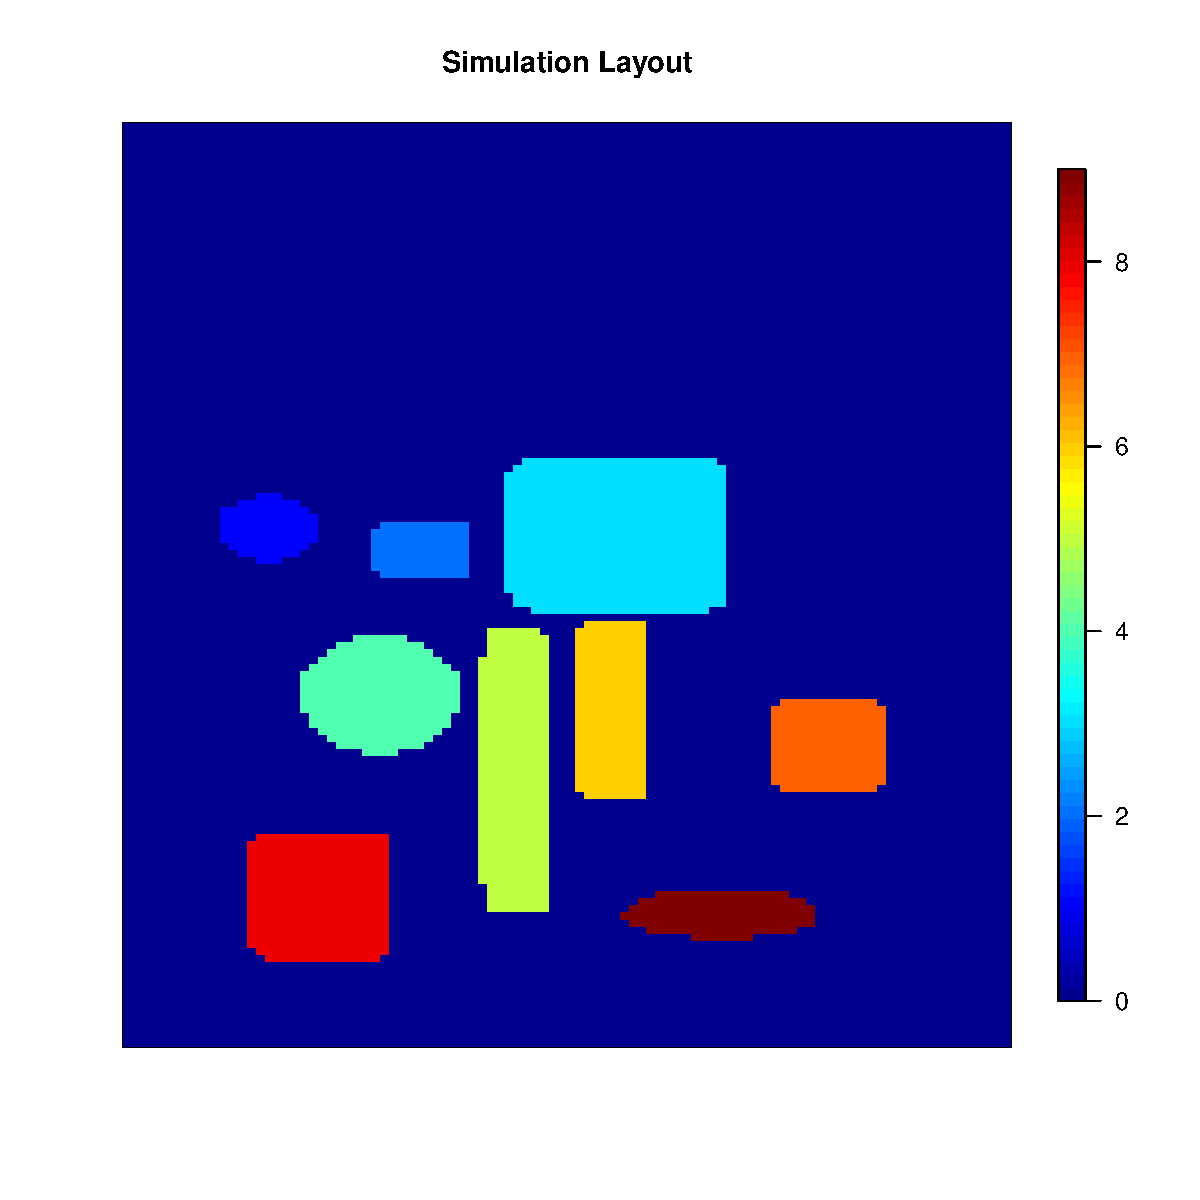
\includegraphics[width = 2.0in]{hsi.pdf}
\caption{Layout for HSI simulations.}
\label{FIG:HSI_IMG}
\end{center}
\end{figure}
 
\begin{figure*}
\begin{center}
\includegraphics[width = 6.5in]{spec_sim2.pdf}
\caption{Plot (a) shows examples of sampled endmembers, plots (b)-(e) show
the corresponding abundances for each with color scale to the right.}
\label{FIG:MIX}
\end{center}
\end{figure*}


\begin{algorithm}[tb]
   \caption{Sampling scheme for endmember generation}
   \label{ALG:EGEN}
\begin{algorithmic} 
   \STATE {\bfseries Define:} 
   \begin{enumerate}
     \item  $f_j(\mathbf{x})$ to be one of $\sin(\mathbf{x})$,
     $\cos(\mathbf{x})$, $\mathbf{x}$, $\mathbf{x}^2$, $\tanh(\mathbf{x})$, $\mathbf{x}^3$, $1/\mathbf{x}$, $\exp(-\mathbf{x}^2)$, $\sinh(\mathbf{x})$,
   $\cosh(\mathbf{x})$ where $j=1$ corresponds to $\sin(\mathbf{x})$, $j=2$ is
   $\cos(\mathbf{x})$, etc. Here  $f_j(\mathbf{x})$
   is the $j^{th}$ functions evaluated for each element in $\mathbf{x}\{-2\pi +
   i\pi/25 \}_{i=1}^{100}$.
   \item  $scale(\mathbf{x}) = \mathbf{x} -
   \min\{\mathbf{x}\}/(\max\{\mathbf{x}\} - \min\{\mathbf{x}\}).$
   \end{enumerate} 
%       $f_1(\mathbf{x}) = \sin(\mathbf{x})$,
%       $f_2(\mathbf{x}) = \cos(\mathbf{x})$,
%       $f_3(\mathbf{x}) = \mathbf{x}$,
%       $f_4(\mathbf{x}) = \mathbf{x}^2$,
%       $f_5(\mathbf{x}) = \tanh(\mathbf{x})$,
%       $f_6(\mathbf{x}) = \mathbf{x}^3$, 
%       $f_7(\mathbf{x}) = 1/\mathbf{x}$, 
%       $f_8(\mathbf{x}) = \mbox{exp}(-\mathbf{x}^2)$,
%       $f_9(\mathbf{x}) = \sinh(\mathbf{x})$,
%       $f_{10}(\mathbf{x}) = \mathbf{cosh}(\mathbf{x})$,
   \STATE {\bfseries Iterate:} Until 10 unique endmembers have been generated
   \begin{enumerate}
\item Take a random sample without replacement of size $R \in \{1,2,3\}$ from
$\{1,\ldots,10\}$ call this sample $S$.
\item Compute endmembers as $\mathbf{X}_i = scale\left(\bigotimes_{j \in S}
scale(f_j(\mathbf{x}))\right)$, where $\bigotimes$ is the elementwise
product. 
\end{enumerate}
   \STATE {\bfseries Output:} Endmember matrix $\mathbf{X} = (\mathbf{X}_1,
   \ldots, \mathbf{X}_{10}) \in \mathbb{R}^{100 \times 10}$.
\end{algorithmic}
\end{algorithm}

 
The objective of this simulation study is two-fold; first, to see if we are able
to identify the proper subset of endmembers and second, assess the accuracy of
the abundance estimates. We also look at the impact that varying the levels of
noise $\sigma$ and correlation between endmembers has on performance.
Regarding the latter we consider two scenarios; first, in Algorithm
\ref{ALG:EGEN} an endmember is added to the dictionary only if its correlation
(in absolute value) is less than 0.7 with any other endmember already in the
dictionary, and second if the correlation is greater than 0.6.
% Looking at varying levels of correlation is of interest as it highlights the
% the ridge-regression like behavior that the group-sparse and spatial
% constraints have on the coefficient estimates.
% In particular when variables (endmembers) are highly correlated the ridge-type
% penalty will ``encourage'' their coefficients estimates to be the same.
% In the context of trying to identify the true subset of endmembers from a
% larger dictionary if a signal endmember is strongly correlated with a noise
% endmember, oftentimes the effect is that both are kept in the model.


We compare three models, the GL, SGL and SSGL.
For all methods we use an adaptive penalty for the group sparse parameters.
Specifically, we fit a non-negative least squares model to the data with
associated coefficient estimates $\hat{\mathbf{B}}_{nnls} \in \mathbb{R}^{8000
\times 10}$ and use $\omega_j = \sum_{k=1}^{8000} (\beta^{(k)}_j(nnls))^2$, $j =
1,\ldots,10$ as the weights.
The final group regularization parameters are computed as $\lambda_j =
\lambda/\omega_j$. We found that for these simulations $\lambda$ equal to 5 and
1 worked best for the GL and SGL models respectively and for SSGL 2.5 worked
best for the low correlation case and 0.5 for the high
correlation case.

For the SSGL model neighborhood size is fixed at 1 and the cutoff for
the cosine similarity (discussed in Section \ref{SEC:SPLASSO}) is 0.95.
Additionally, for the low and high correlation cases we found that a spatial
regularization parameter of $\rho = 0.75$ and $0.1$ respectively worked well. 

Also, note that in order to satisfy the non-negatively constraints for the
coefficient estimates (discussed in Section \ref{SEC:INTRO}) we simply modify
Step 3 in the iteration step of Algorithm \ref{ALG:BCD} to set
$\hat{\beta}_j^{(k)} = 0$ when $S(b_j^{(k)}, \gamma_k) < 0$.

The results, shown in Table \ref{TAB:HSI_RES} are the sums of squares error
(SSE) across the $K = 8000$ pixels between the estimated abundances (the
$\hat{\beta}_j^{(k)}$'s for each model) and the actual abundances (shown in
Figure \ref{FIG:MIX} (e)-(h)). The columns with corr $< 0.7$ and $> 0.6$
correspond to the low and high correlation cases respectively. Within each of
these the columns titled 0.05 and 0.1 are the associated values of $\sigma$ and
beneath these are the SSEs. 

These results show the overall strong performance of the SSGL model relative to
the GL and SGL. Additionally, with the exception of the SGL model none of the
methods ever selected a non-signal endmember, however, some failed to select
endmembers actually present in the model. In the case of the latter an ``NA'' is
reported.
For the SGL model there was one instance where an additional non-signal
endmember was selected (for corr $< 0.7$ and $\sigma = 0.1$).

An important feature of these models highlighted by the results in Table
\ref{TAB:HSI_RES} is the considerable impact that increased correlation between
variables has on performance. Specifically, the drastic increase in SSEs for all
methods and in particular for the SSGL.
For the SSGL model receives this is largely driven by the ridge-like penalty it
receives from both the group and spatial penalty parameters. The result is an
increase in the degree to which highly correlated variables ``collapse'' to the
same value. This once again highlights the importance of balancing group and
spatial penalty terms in training our model.



\begin{table}
\begin{center}
\renewcommand{\arraystretch}{0.9}
\begin{tabular}{|c|c|c|c|c|c|}
\hline
 & & \multicolumn{2}{|c|}{$\mbox{corr} < 0.7$} &
 \multicolumn{2}{|c|}{$\mbox{corr} > 0.6$}\\
\hline
Model & Endm. & $0.05$ & $0.1$ & $0.05$ & $0.1$ \\
\hhline{|=|=|=|=|=|=|}
\multirow{4}{*}{GL} 
&	1	&	8.87	&	12.42	&	38.43	&	81.08	\\
&	2	&	2.2	&	8	&	217.42	&	92.57	\\
&	3	&	0.77	&	1.31	&	NA	&	NA	\\
&	4	&	1.87	&	19.19	&	NA	&	27.24	\\
\hhline{|=|=|=|=|=|=|}
\multirow{4}{*}{SGL} 
&	1	&	9.35	&	8.16	&	25.1	&	42.87	\\
&	2	&	1.5	&	3.81	&	217.21	&	118.68	\\
&	3	&	0.56	&	1.31	&	NA	&	NA	\\
&	4	&	0.98	&	5.79	&	88.01	&	12.85	\\
\hhline{|=|=|=|=|=|=|}
\multirow{4}{*}{SSGL} 
&	1	&	8.44	&	4.58	&	29.96	&	40.17	\\
&	2	&	1.41	&	1.77	&	200.49	&	95.34	\\
&	3	&	0.13	&	0.26	&	150.82	&	NA	\\
&	4	&	0.42	&	3.43	&	89.14	&	7.72	\\
\hline
\end{tabular}
\caption{SSEs of estimated endmember abundances for
simulated HSI image.}
\label{TAB:HSI_RES}
\end{center}
\end{table}


\subsection{Microscene Experiment}
Following a similar method of analysis as in \cite{sgen2014} we provide results
on the analysis of a ``microscene'' experiment, originally presented in
\cite{allen2013}. The purpose of this experiment is to provide a protocol for
assessing the performance of hyperspectral imaging cameras and algorithms for
detecting/classifying various substances. The physical object being imaged is a
petri dish which contains a mix of things like sand, parsley, copper, etc. The
idea is to recreate the complexity of remotely sensed data (e.g. captured via
plane, drone and/or satellite). With such an object hyperspectral cameras can
then be appropriately calibrated to ensure that they are able to detect all the
substances present in the scene before being sent out into the real world.

The microscene used in our analysis is shown in Figure \ref{FIG:PETRI} (a) which
contains 14 unique (many of which are highly correlated) substances whose
spectra are shown in Figure \ref{FIG:PETRI} (b). To test the SGL and the SSGL
algorithms ability to detect the correct subset of endmembers (we focus on these
two for purposes of space) from a larger dictionary of endmembers we choose a
subset of the image to analyze, shown in Figure \ref{FIG:PETRI} (c), which
contains 5 of the 14 substances.

\begin{figure*}
\begin{center}
\includegraphics[width = 5in]{petri.png}
\caption{Test scene for analyzing hyperspectral remote sensing measurements.}
\label{FIG:PETRI}
\end{center}
\end{figure*}
 
As no ground truth is available it is difficult to provide a direct quantitative
measure as to how well the abundances of these substances have been estimated,
so aside from correctly identifying the number of substances our analysis here
is largely qualitative. The results are shown in Figures \ref{FIG:MSGL} and
\ref{FIG:MSSGL} for the SGL and SSGL models respectively.
 
Each figure contains the abundance (i.e. coefficient) estimates for each
endmember identified as being present by each model in the subregion of
interest. Along the x-axis is an index for which endmember was found and the
heatmaps show the associated abundance estimates at each pixel.
Both approaches identify the same subset of 5 endmembers.

One of the endmembers identified, endmember 2, is {\it not} in the subregion.
However, it is very strongly correlated ($> 0.99$) with endmember 13, which is
the actual substance present, yet neither model selected the latter. We believe
that this could be a result of the ridge-like behavior of the $l_2$ group
penalty, and/or an artifact of the deterministic nature of the CBD algorithm. As
part of future work we plan to look into the use of stochastic coordinate
descent (\cite{shwartz2011}) in place of CBD which could partially alleviate
this issue.

As expected the SSGL model produces smooth coefficient estimates whereas the SGL
model has coarser estimates. One could argue that the distribution of the
substances in any given region should be fairly uniform so the smooth estimates
of the SSGL may be more appropriate. However, that being said the
inclusion of the smoothing penalty also causes the estimated abundances to
shrink (in particular for endmembers 2 and 10), giving the appearance of
``less'' of that substance.
Both models had a difficult time capturing the abundances associated with
endmember 10. This could be due in
part to the ``salt and pepper'' nature of the region (see Figure \ref{FIG:PETRI}
(a)).

\begin{figure}[h!]
\begin{center}
\includegraphics[width = 2.0in]{sgl_res_roi.png}
\caption{SGL results for microscene experiment}
\label{FIG:MSGL}
\end{center}
\end{figure}

\begin{figure}[h!]
\begin{center}
\includegraphics[width = 2.0in]{ssgl_res_roi.png}
\caption{SSGL results for microscene experiment}
\label{FIG:MSSGL}
\end{center}
\end{figure}
%%=============================================================================
 \bibliographystyle{bka}
 \bibliography{sgen}
%%=============================================================================
 
\end{document}